\section{Introduction}

Since its proposal, the lasso \citep{tibshirani_1996} has become an immensely popular modeling approach due to its ability to simulataneously achieve variable selection and estimation via penalization. In the usual linear regression setting, the lasso models an $n$-dimensional vector of continuous outcomes, $\y$, as a linear combination of covariates contained in an $n$ by $p$ design matrix, $\X$, and a $p$-dimensional vector of regression coefficients, $\bb$, with an $l_1$ penalty imposed on the size of $\bb$. More precisely, the lasso estimator of $\bb$ is defined as the minimizer of:
\begin{equation*}
Q_{\text{lasso}}(\bb) = \tfrac{1}{2n}||\y - \X\bb||^2 + \lam||\bb||_1
\end{equation*}
Perhaps the most desirable property of the lasso is that some components of $\bbh$ are estimated to be exactly 0 for sufficiently large values of the penalty parameter, $\lambda$, implying the remaining non-zero elements have been \textit{selected} by the lasso.  Unfortunately, selections made by the lasso can be unsatisfactory in applications involving categorical predictors.  In these circumstances, the lasso willl select amongst the individual dummy variables rather than the underlying predictors themselves, thereby making selections dependent upon the scheme used to encode the dummy variables and complicating efforts to identify and interpret impactful categorical predictors.  The lasso faces a similar barrier in applications where basis expanasions are used to represent non-linear additive effects of predictors, as the overall selection status of an underlying predictor can be unclear if some columns of the basis expansion are selected but others are not.

The group lasso \citep{Yuan2006} is capable of addressing these shortcomings by imposing an $l_2$ penalty upon groups of coefficients, rather than individual coefficients, thus resulting in selections occuring at the group level.  For linear regression applications, the group lasso estimator of $\bb$ is defined:
\begin{equation*}
Q(\bb) = \tfrac{1}{2n}||\y - \X\bb||^2 + \sum_{j = 1}^{J}\lambda_j ||B_j||
\end{equation*}
The penalization scheme employed by the group lasso has since been extended to many generalized linear models, with logistic regression \citep{meier2008} serving as a notable example among many others.

A potential drawback of the group lasso is the limited scope of inferential methods available after model fitting.  While the recently developed \textit{selective inference} \citep{Selective_Inference} family of methods has been extended to group sparse settings, including the group lasso \citep{Yang2016}, a software implementation is only available for forward stepwise selection.  Similarly, the \textit{knockoff filter} method of false discovery rate control \citep{barber2015, candes2018} has also been extended to group sparse settings \citep{Dai2016}, but it too lacks an available software implementation for group lasso models.  Meanwhile, computational inferential approaches with readily available software, such as the parametric bootstrap approach implemented in the {\tt EAinference} R Package \citep{Zhou2017}, focus on the uncertainty in the individual coefficient estimates found using the group lasso, rather than the selections of entire groups.

The focus of this paper is on the reliability of group level selections made by the group lasso and its variants.  More specifically, we propose methods for controlling the marginal false discovery rate of group selections in the context of group lasso regression.  Our proposed methods provide computationally efficient alternatives to the limited set of existing inferential approaches for the group lasso.  We demonstrate the robustness of these methods across a variety of data structures, as well as their ability to achieve higher true positive rates than existing inferential approaches.  Further, we generalize our methods to extensions of the group lasso, including logistic regression and other generalized linear models, as well as non-convex group penalization schemes \citep{Breheny2012}.



\section{Background}

\subsection{Group lasso regression}

Consider data of the usual form, $(\y, \X)$, where $\y$ records the response values of $i \in \{1, \ldots, n\}$ independent observations, and $\X$ is an $n$ by $p$ design matrix of explanatory variables.  We focus on situations in which the columns of $\X$ can be naturally placed into $J$ nonoverlapping groups, such that $\X = \{\X_1, \X_2, \ldots, \X_J\}$, where $\X_j$ denotes the $n$ by $K_j$ matrix containing the explanatory variables belonging to group $j$.  

The explanatory variables in $\X$ can be related with $\y$ using a probability model involving a set of coefficients, $\bb$.  A well-known example is the linear regeression model, which specifies the relationship:
\begin{equation}
\label{m:lin}
\y = \X\bb + \beps
\end{equation}
where $\beps$ is a vector of independent, Normally distributed errors, with mean 0 and variance $\sigma^2$. 

Under the model described in \ref{m:lin}, the group lasso solution, $\bbh$, is defined as the minimize, with respect to $\bb$, of the group lasso objective function, denoted $Q(\bb)$:
\begin{equation}
Q(\bb) = \tfrac{1}{2n}||\y - \X\bb||^2 + \sum_{j = 1}^{J}\lambda_j ||\beta_j||
\end{equation}
where $\lambda_j$ is a penalty applied to $l_2$-norm of the coefficients in group $j$.  While it is possible to specify $\lambda_j$ individually for each group, the more common choice is to penalize in accordance to group size by setting $\lambda_j = \sqrt{K_j}\lambda$, where $\lambda$ is universal across groups. 

The underlying framework of the group lasso can be generalized to a wide range of loss functions and penalization schemes whose solutions minimize the following objective function:
\begin{equation}
Q(\bb) = L(\bb|\X,\y) + \sum_{j = 1}^{J} p_{\lambda}(\bb_j)
\end{equation}
where $p_{\lambda}(\cdot)$ is a penalty function applied to each group of coefficients, and $L(\bb|\X,\y)$ is a loss function, which is upon the log-likelihood in the case of generalized linear models.  See \citet{Huang2012} for selective review of other grouped penalization schemes.

For sufficiently large $\lambda_j$, the entire group of coefficients belonging group $j$ will all be estimated as exactly zero, making it possible to use the group lasso to perform variable selection at the group level.  Throughout the remainder of this paper, we refer to groups whose group lasso coefficient estimates are non-zero as being ``selected" by the group lasso.  The group lasso penalty has the added benefit of shrinking coefficient estimates towards zero, therefore allowing identifiable estimation even when the dimensionality of $\X$ is such that $p > n$.

In their original proposal, \citet{Yuan2006} assume the data have been orthonormalized within each group, such that $\tfrac{1}{n}\X_j^T\X_j = \I$ for all $j \in \{1, \ldots, J\}$ with $\I$ representing the identity matrix, prior to model estimation.  Although data are unlikely to naturally occur in this form, groups can be orthonormalized as a pre-processing step.  Provided $K_j < n$ for all $j \in \{1, \ldots, J\}$, any optimization done using the orthonormalized data is equivalent to the original scale.  Further, the group lasso solution of the orthonormal scale can also be easily converted back to the orginal scale.  Throughout the remainder of this paper we assume the data have already been orthonormalized within in each group as a pre-processing step. See \citet{Simon2012} for further discussion of this topic.


\subsection{Marginal false discovery rates}

The work of \citet{BH_1995} has led to false discovery rate (FDR) control becoming perhaps the most widely utilized inferential paradigm in applications involving large numbers of simulataneous comparisons between variables.  The literature on false discovery rate control is enormous, with many authors operating under slightly different definitions.  One straightfoward way to characertize the false discovery rate is as the expected number of false selections divided by the total number of selections, or as the fraction of significant features that are false positives.  In this regard, a selection procedure that controls the FDR at 10\% corresponds to the expectation that no more than 10\% of the comparisons it identifies as siginificant are expected to be false positives.  

Much of the work in the realm of false discovery rate control pertains to \textit{large scale univariate testing}, or applications that entail the aggregation of results of a large number of single variable hypothesis tests, \citet{Farcomeni2008} and \citet{Strimmer2008} provide a more detailed overview of these methods.  In the regression modeling framework, the notion of a false discovery can be considerably more complicated in the presence of relationships between predictors.  To better understand these complexities, consider the causal diagram shown below, which illustrates a possible relationship between three explanatory variables, $A$, $B$, and $C$, and an outcome variable $Y$.

%\begin{figure}[!htb]
%\centering
\begin{center}
\begin{tikzpicture}[node distance=1cm]

% nodes %
\node(b)[text centered] {$B$};
\node(u)[below of = b, text centered] {$ $};
\node(a)[left of = u,  text centered, xshift = -1.5cm] {$A$};
\node(c)[right of = u, text centered, xshift = 1.5cm] {$C$};
\node(y)[below of = u, text centered] {$Y$};
 
% edges %
\draw [arrow] (a) -- (b);
\draw [arrow] (a) -- (y);

\end{tikzpicture} \\
\end{center}
%\caption{\label{Fig:diagram} Causal diagram showing three types of relationships between variables and the outcome.}
%\end{figure}

In this scenario, variable $A$ has a direct causal relationship with $Y$ and should never be considered a false discovery, while variable $C$ is independent of $Y$ and should always be considered a false discovery.  Whether or not variable $B$ should be considered a false discovery less clear.  According to the paradigm used in large scale univariate testing, variable $B$ would not be seen as a false discovery because it is not \textit{marginally independent} of variable $Y$, the criteria that is typically considered in each single variable hypothesis test.  Alternatively, in the regression setting, the coefficient in the data generating model corresponding to variable $B$ would be zero, suggesting that variable $B$ should be viewed as a false discovery.  In the context of group selections, the underlying idea conveyed by this causal structure can be generalized such that $A$, $B$, and $C$ represent groups of variables acting in concert.

To further clarity these distinctions, we introduce two contrasting false discovery rate perspectives: the \textit{marginal} perspective, in which the variable, or group of variables, denoted $X_j$ is a false discovery if it is declared significant despite being fully indpendent of the outcome: $\X_j \independent Y$, and the \textit{fully conditional} perspective, where $X_j$ is a false discovery if it is deemed significant despite being independent of the outcome conditional upon all of the other variables in the data: $X_j \independent Y | X_{k \neq j}$.  Because penalized regression methods, including as the group lasso, allow for only a subset of the available predictors to be active in a given model, a \textit{pathwise conditional} perspective is also possible.  This perspective focuses on the model where $X_j$ first becomes active and conditions only on the other variables present in the model (a set we denote $M_j$) at that time when assessing whether or not variable $j$ is a false discovery: $X_j \independent Y | X_k \text{ for } k \in M_j$.

The methods developed in this paper utilize the less restrictive \textit{marginal false discovery rate} definition.  While the selection of variables like $B$ in the aforementioned causal diagram can be problematic in certain applications, in most applications it is impossible to untangle the true causal structure of the $A-B-Y$ relationship, and it is universally useful, regardless of application, to control the number of variables like $C$ that are deemed significant.  For these reasons, as well as the existing adoption of the marginal definition within the realm of large scale univariate testing, we argue the marginal false discovery rate is a valuable quantity to consider in applications involving the group lasso.  Furthermore, marginal false discovery rate inferential approaches have gained traction in recent years, with \citet{Breheny2019, Miller2019, Liang2021} developing methods for the ordinary lasso, penalized GLMs and survival models, and penalized transformation models respectively.

\section{Marginal false discovery rates for the group lasso}

\subsection{Linear regression}

Consider data arising from the usual linear model:
\begin{equation}
\y = \X\bb + \beps
\end{equation}
where $\beps \sim N(\zero, \sigma^2\I)$ and $\X$ is presumed to have a known grouping structure such that $\bb_j$ is a vector of length $K_j$ representing the regression coefficients associated with group $j \in \{1, \ldots, J\}$.  Our goal is to characterize the expected number and rate falsely selected groups for a given group lasso model.

We begin with the group lasso solution, $\bbh$, which is defined as the minimizer of the group lasso objective function, $Q(\bb)$:
\begin{equation}
Q(\bb) = \tfrac{1}{2n}||\y - \X\bb||^2 + \sum_{j = 1}^{J}\lambda_j ||B_j||
\end{equation}
Solving for $\bbh$ requires the subdifferential (cite Bertsekas 1999) of $Q$ with respect to $\bb_j$:
\begin{equation}
  \label{eq:kkt}
  \begin{alignedat}{2}
  -\tfrac{1}{n}\X_j^T(\y - \X_{-j}\bb_{-j}) + \bb_j + \lambda_j\tfrac{\bb_j}{||\bb_j||}  &\quad \text{if } \bb_j &\neq 0 \\
  -\tfrac{1}{n}\X_j^T(\y - \X_{-j}\bb_{-j}) + \lambda_j\mathbf{v}  &\quad \text{if }  \bb_j &= 0
  \end{alignedat}
\end{equation}

Here, $\mathbf{v}$ is any vector satisfying $||\mathbf{v}|| < 1$, and the notation $\X_{-j}$ is used to denote the portion of $\X$ that remains after removal of the covariate group contained in $\X_j$, with $\bb_{-j}$ describing the associated model coefficients.  In the optimzation literature, the criteria described in \ref{eq:kkt} are known as the KKT conditions.  

It follows from these conditions that if the $j^{th}$ group is to be selected into the model with non-zero coefficients, it must be that the case that:
\begin{equation}
  \label{eq:post_ktt}
\tfrac{1}{n}\X_j^T(\y - \X_{-j}\bbh_{-j}) - \bbh_j = \lambda_j\tfrac{\bbh_j}{||\bbh_j||}
\end{equation}
Thereby prompting the following theorem.

\begin{theorem}
\label{Thm:main}
For the group lasso solution $\bbh$, the component $\bbh_j \ne \zero$ if and only if

\begin{equation}
  \label{eq:selc}
\tfrac{1}{n}||\X_j^T(\y - \X_{-j}\bbh_{-j})||^2 > \lambda_j^2
\end{equation}

Further, given the group $\X_j$ is marginally independent of $\y$, if $\tfrac{1}{n}\X_j^T \X_{-j}^T \inP \zero$ and $\lambda$ is chosen such that $\sqrt{n}(\bbh -  \bb)$ is bounded in probability, then
\begin{equation}
  \label{eq:thm1}
  \tfrac{1}{n \sigma^2}||\X_j^T(\y - \X_{-j}\bbh_{-j})||^2 \inD \chi^2_{K_j}
\end{equation}
\end{theorem}

\begin{proof}
The first statement is a straightfoward algebraic manipulation of \ref{eq:post_kk}, which is a direct consequence of the KKT conditions in \ref{eq:kkt}.  Then, expanding the left side of Expression~\ref{eq:selc} yields:
\begin{align}
\begin{alignedat}{2}
\tfrac{1}{n}||\X_j^T(\y - \X_{-j}\bbh_{-j})||^2 &= \tfrac{1}{n}||\X_j^T(\X\bb + \beps - \X_{-j}\bbh_{-j})||^2 \\
                                                     &= \tfrac{1}{n}||\X_j^T\beps - \X_j^T\X_{-j}(\bb_{-j} - \bbh_{-j})||^2 
\end{alignedat}
\end{align}
Noting $\tfrac{1}{\sqrt{n}} \X_j^T\X_{-j}(\bb_{-j} - \bbh_{-j}) \inP \mathbf{0}$ and $\beps \sim N(\zero,\sigma^2\I)$, we have $\tfrac{1}{n \sigma^2}||\X_j^T(\y - \X_{-j}\bbh_{-j})||^2 \inD \chi^2_{K_j}$.
\end{proof}

The first condition of Theorem~\ref{Thm:main}, $\tfrac{1}{n}\X_j^T \X_{-j}^T \inP \zero$, can be satisified when correlations between the columns belonging to group $j$ and the others in $\X$ become neglible as $n$ increases. While the second condition, that $\sqrt{n}(\bbh -  \bb)$ is bounded in probability, is met for suitable choices of $\lambda$ (CITE http://proceedings.mlr.press/v5/liu09a/liu09a.pdf).   

The first condition is not a trivial assumption; however, it represents a valuable worst-case scenario in regards to false discoveries.  Heuristically, in penalized regression applications where two groups are related the selection of one group decreases the chances that the other is also selected, thereby leading to fewer chance selections than would be expected had there been no relationship across groups.  Characterizing the precise degree of conservatism induced in these scenarios is siginificantly less mathematically tractable, but we extensively explore the issue via simulation study in section (REF sim).  (CITE BREHENY 2019) provides a more detailed theoretical discussion in the context of the ordinary lasso.

\begin{clry}
Under the conditions outlined in Theorem~\ref{Thm:main}, for the group lasso model characterized by $\lambda$, the expected number of false discoveries and the expected rate of marginal false discoveries are respectively bounded by:
\begin{align}
  \label{eq:Mfdr}
  \begin{alignedat}{2}
\FD &= \sum_{j = 1}^{J} \Pr \big(\chi^2_{K_j} > \frac{n\lam_j^2}{\sigma^2}\big)\\
\mFDR  &= \frac{\FD}{\text{S}} 
  \end{alignedat}
\end{align}
where $\text{S}$ denotes the total number of selected groups in the model defined by $\lambda$.
\end{clry}

Theorem~\ref{Thm:main} implies the probability that the $j^{th}$ group is selected, given the group is marginally independent of the outcome, corresponds to the probability that a $\chi^2_{K_j}$ random variable is larger than $\frac{n\lam_j^2}{\sigma^2}$.  In principle, we'd then sum over all groups that are marginally indpendent of the outcome to determine the expected number of falsely selected groups; however, the identity of such groups is unknown in practice, so summing over all $J$ groups provides a conservative alternative.  In many applications of the group lasso, the number of groups that are truly related to the outcome tends to be small relative to the total number of groups, making this effect relatively small.

For a given value of $\lambda$, the process of calculating $\mFDR$ is summarized in Algorithm~\ref{Alg:mfdr}.

\begin{algorithm*}
\caption{Calculating the mFDR upper bound}\label{Alg:mfdr}
\begin{algorithmic}[10]
\Procedure{}{}
	\State Estimate $\sigma^2$ as either $\hat{\sigma}^2 = \frac{\rr^T\rr}{n - df}$ or $\hat{\sigma} = \text{cve}_{\lambda}$
	\For {\texttt{$j \in \{1, \ldots, J\}$}}
		\State $\widehat{\FD}_{j, \lam} = \Pr \big(\chi^2_{K_j} > \frac{n\lam_j^2}{\hat{\sigma}^2}\big)$  by the result of Theorem 1
	\EndFor
	\State $\widehat{\FD}_\lam =  \sum_{j=1}^{J} \widehat{\FD}_{j, \lam} $
	\State $\widehat{\mFDR}_\lam = \text{min}\left(\frac{\widehat{\FD}_\lam}{S_\lam}, 1 \right)$
\EndProcedure
\State \textbf{return} $\widehat{\mFDR}_\lam $
\end{algorithmic}
\end{algorithm*}

We point out that the initial step of Algorithm~\ref{Alg:mfdr} requires estimating $\sigma^2$, either by dividing the residual sum of squares by its degrees of freedom or taking it to be the cross-validated error of the model under consideration.  

\subsection{Generalized linear models}

The penalization scheme of the group lasso can be extended to other likelihood-based models, notably those corresponding to various generalized linear models (GLMs).  In these settings, a quadratic approximation of the log-likelihood function, $L$, is typically used in solving for the group lasso coefficients:
\begin{equation}
L(\be) = L(\bet) + (\be - \bet)^T\vv + \tfrac{1}{2}(\be - \bet)^T\W(\be - \bet)
\end{equation}
where $\eta = \X\bb$, with $\bet$ denoting the current estimate, and $\vv$ and $\W$ respectively represent the first and second derivatives of $L(\be)$ evaluated at $\bet$.  It is worthwhile noting that $\W$ is a diagonal matrix in popular GLMs such as logistic regression.  Letting $\z = \bet - \W^{-1}\vv$, and dropping terms that are constant with respect to $\bb$, this approximation yields a loss function that is equivalent to weighted squared error loss:
\begin{equation}
L(\bb) \approx \tfrac{1}{2}(\z - \X\bb)^T\W(\z - \X\bb)
\end{equation}
Thus, the optimization algorithms that solve for the group lasso solution, as well as their corresponding KKT conditions, can be adapted to generalized linear models with the minor addition of a weight matrix, $\W$. Consequently, groups selections within these models are characterized by the following condition:
\begin{equation}
  \label{eq:sel_glm}
\tfrac{1}{n}||\X_j^T\W(\z - \X_{-j}\bbh_{-j})||^2 > \lambda_j^2
\end{equation}
Applying the same general steps used in the linear regression setting, we can work towards characterizing the marginal false discovery rate of these models using the left hand side of expression~\ref{sel_glm}:
\begin{equation}
  \label{eq:Mfdr_proof_glm}
\tfrac{1}{n}||\X_j^T\W(\z - \X_{-j}\bbh_{-j})||^2 = \tfrac{1}{n}||\X_j^T\vv - \X_j^T\W\X_{-j}(\bb_{-j} - \bbh_{-j})||^2 
\end{equation}

\begin{prop}
\label{prop1}
Provided $(\X^T\W\X)^{-1/2}\X^T\vv \inD N(\zero, \I)$, where $\I$ is the $p$ x $p$ identity matrix,  $\tfrac{1}{n}\X_j^T \W \X_{-j}^T \inP \zero$, and $\sqrt{n}(\bbh-  \bb)$ is bounded in probability.  The number and rate of marginal false discoveries in likelihood-based models subjective to the group lasso penalty can be characterized as follows:
\begin{align}
  \label{eq:Mfdr_glm}
  \begin{alignedat}{2}
\FD &= \sum_{j = 1}^{J} \Pr \bigg(\chi^2_{K_j} > \frac{n^2\lam_j^2}{\Tr(\X_j^T\W\X_j)}\bigg)\\
\mFDR  &= \frac{\FD}{\text{S}} 
  \end{alignedat}
\end{align}
\end{prop}

The first condition involved in \ref{prop1} is a standard result of classical likelihood theory which can be shown for many types of generalized linear models, while the other two conditions are direct analogs of those in \ref{Thm:main} for the linear regression setting.  Consequently, the underlying derivation giving rise to the estimates in \ref{eq:Mfdr_glm} is analgous to that of Theorem~\ref{Thm:main}, with the primary difference being that the variance used in normalization.  Like before, we can summarize the procedure involvied in calculating $\mFDR$ for given value of $\lambda$ using the following algorithm:

\begin{algorithm*}
\caption{Calculating the mFDR upper bound (GLMs}\label{Alg:mfdr_glm}
\begin{algorithmic}[10]
\Procedure{}{}
	\State Estimate $\widehat{W} \gets \nabla^2f(\beh)$
	\For {\texttt{$j \in \{1, \ldots, J\}$}}
		\State $\widehat{\FD}_{j, \lam} = \Pr \bigg(\chi^2_{K_j} > \frac{n^2\lam_j^2}{\Tr(\X_j^T\W\X_j)}\bigg)$ by Proposition 1
	\EndFor
	\State $\widehat{\FD}_\lam =  \sum_{j=1}^{J} \widehat{\FD}_{j, \lam} $
	\State $\widehat{\mFDR}_\lam = \text{min}\left(\frac{\widehat{\FD}_\lam}{S_\lam}, 1 \right)$
\EndProcedure
\State \textbf{return} $\widehat{\mFDR}_\lam $
\end{algorithmic}
\end{algorithm*}

As was the case in the linear regression setting, the estimates arising from \ref{Alg:mfdr_glm} will be conservative in the presence of correlations between explanatory variables, or in applications were $J$ is substantially greater than the number of groups that are marginally independent of the outcome.  Additionally, these estimates are subject to added uncertainty from the use of the average diagonal element of $\X_j^T\W\X_j$ in normalization.  In Section~\ref{Sec:sim} we demonstrate the reliability of these estimates when applied to group lasso logistic regression.


\subsection{Other penalty functions}

The general form of the Mfdr estimator in \ref{eq:Mfdr} is directly applicable to a number of other penalizations schemes that are related to the group lasso.  One example is the minimax concave penalty, or MCP, whose penalty function, $f_{\lambda, a}(\theta)$, is defined by
\begin{equation}
  \label{eq:mcp}
  \begin{alignedat}{2}
  \lambda\theta - \tfrac{\theta^2}{2a} &\quad \text{if } \theta &\leq a\lambda \\
  \tfrac{1}{2}a\lambda^2  &\quad \text{if }  \theta &> a\lambda
  \end{alignedat}
\end{equation}
for values of $\lambda \geq 0$, where $a$ is a tuning parameter, with $a = 3$ being typical in software implementations. MCP is a nonconvex penalty where the degree of penalization is diminished, eventually becoming zero, for large coefficients.  In the grouped setting, the composite group MCP estimate \citep{Breheny2012, Huang2012} is the minimizer of
\begin{equation}
Q(\bb) = \tfrac{1}{2n}||\y - \X\bb||^2 + \sum_{j = 1}^{J}f_{\lambda, b}\bigg(\sum_{k=1}^{K_j} f_{\lambda,a}(|\beta_{jk}|)\bigg)
\end{equation}
where the tuning parameter $b$ is typically chosen to be $K_ja\lambda/2$ to ensure that the group level penalty attains its maximum if and only if each of its components are at their maximum.

While the coefficient estimates that arise from group MCP regression may be somewhat different than those of the group lasso, the optimization conditions that describe the entry criteria for groups to become active in the model remains the same.  Consequently, the same estimators proposed in \ref{eq:Mfdr_glm1} and \ref{eq:Mfdr} can also be used to control the marginal false discovery rate in group MCP regression, even though the resulting group selections may differ.  In Section~\ref{Sec:sim} we consider both the group lasso and group MCP penalization schemes when presenting numerical results on simulated data. 


\section{Simulation experiments}
\label{Sec:sim}

\subsection{Data generation}

In all experiments, the covariates stored in the design matrix, $\X$, are derived from numeric values randomly generated from a multivariate normal distribution, $N(0, \Sigma_X)$. The off-diagonal entries of $\Sigma_X$ are used to invoke specific correlation structures between features.  More specifically, we focus on two different correlation structures: Independence - $cor(\x_a \x_b) = 0$, and Autoregressive -  $cor(\x_a, \x_b) = \rho^{|a - b|}$, for all $a, b \in \{i,\ldots,J\}$.  These numeric values are used to construct design matrices for the two primary applications of the group lasso that we choose to focus on, models which involve nominal categorical predictors and non-parametric additive models.  

In the former application, each variable's underlying numeric values are binned into $k$ equally sized groups, which are then expressed in the design matrix via $k$ dummy variables.  Following discretization, outcomes are generated either from the linear model $\y = \X \bb+ \beps$, where $\epsilon_i$ is independently drawn from a $N(0,1)$ distribution, in linear regression applications, or from a Bernouli distribution with $\Pr(y_i = 1) = 1/(1 + exp(-\x_i^T\bb))$ in logistic regression applications.

In the later application, for linear regression scenarios, outcomes are generated directly from the underlying numeric values according to the model $\y = \sum_{j = 1}^{t} f(\x_j) + \beps$, where the function, $f$, defines a non-linear relationship between active features and the outcome, $t$ is a pre-specified number of non-noise features, and $\epsilon_i$ is independently drawn from a $N(0,1)$ distribution.  In logistic regression scenarios, the outcome is drawn from a Bernoulli distribution with $\Pr(y_i = 1) = 1/(1 + exp(- \sum_{j = 1}^{t} f(\x_{ij})))$.  We consider three forms of $f$: Quadratic - $f(X) = X^2$, Piecewise Linear - $f(X) = \tfrac{0.7}{\sqrt{n}}X$ if $X > 0$ and $f(X) = 0$ otherwise, and Periodic - $f(X) = sin(X)$.  Prior to modeling, each feature undergoes a basis expansion with 3 degrees of freedom, thereby yielding a design matrix, $\X$, consisting of $J$ groups of size $k = 3$.

\subsection{False discovery rate control}

The estimators described in Equations~\ref{eq:Mfdr} and \ref{eq:Mfdr_glm} allow for the expected number of false discoveries to be calculated for every model along a the decreasing sequence of $\lambda$ values that is typically returned by software that fits group lasso models.  The curves in (FIG1) display the mean estimated number of marginal false group selections and the mean empirical number of false group selections averaged over 200 simulation repetitions along a fixed, decreasing sequence of $\lambda$ values in the piecewise linear, non-parametric additive model scenario for both linear and logistic regression with $n = 1000$, $J = 100$, and $t = 10$ for three different correlation structures, autoregressive with $\rho \in \{0.5, 0.9\}$, and independence.

\begin{figure} [!htb]
 \centering
  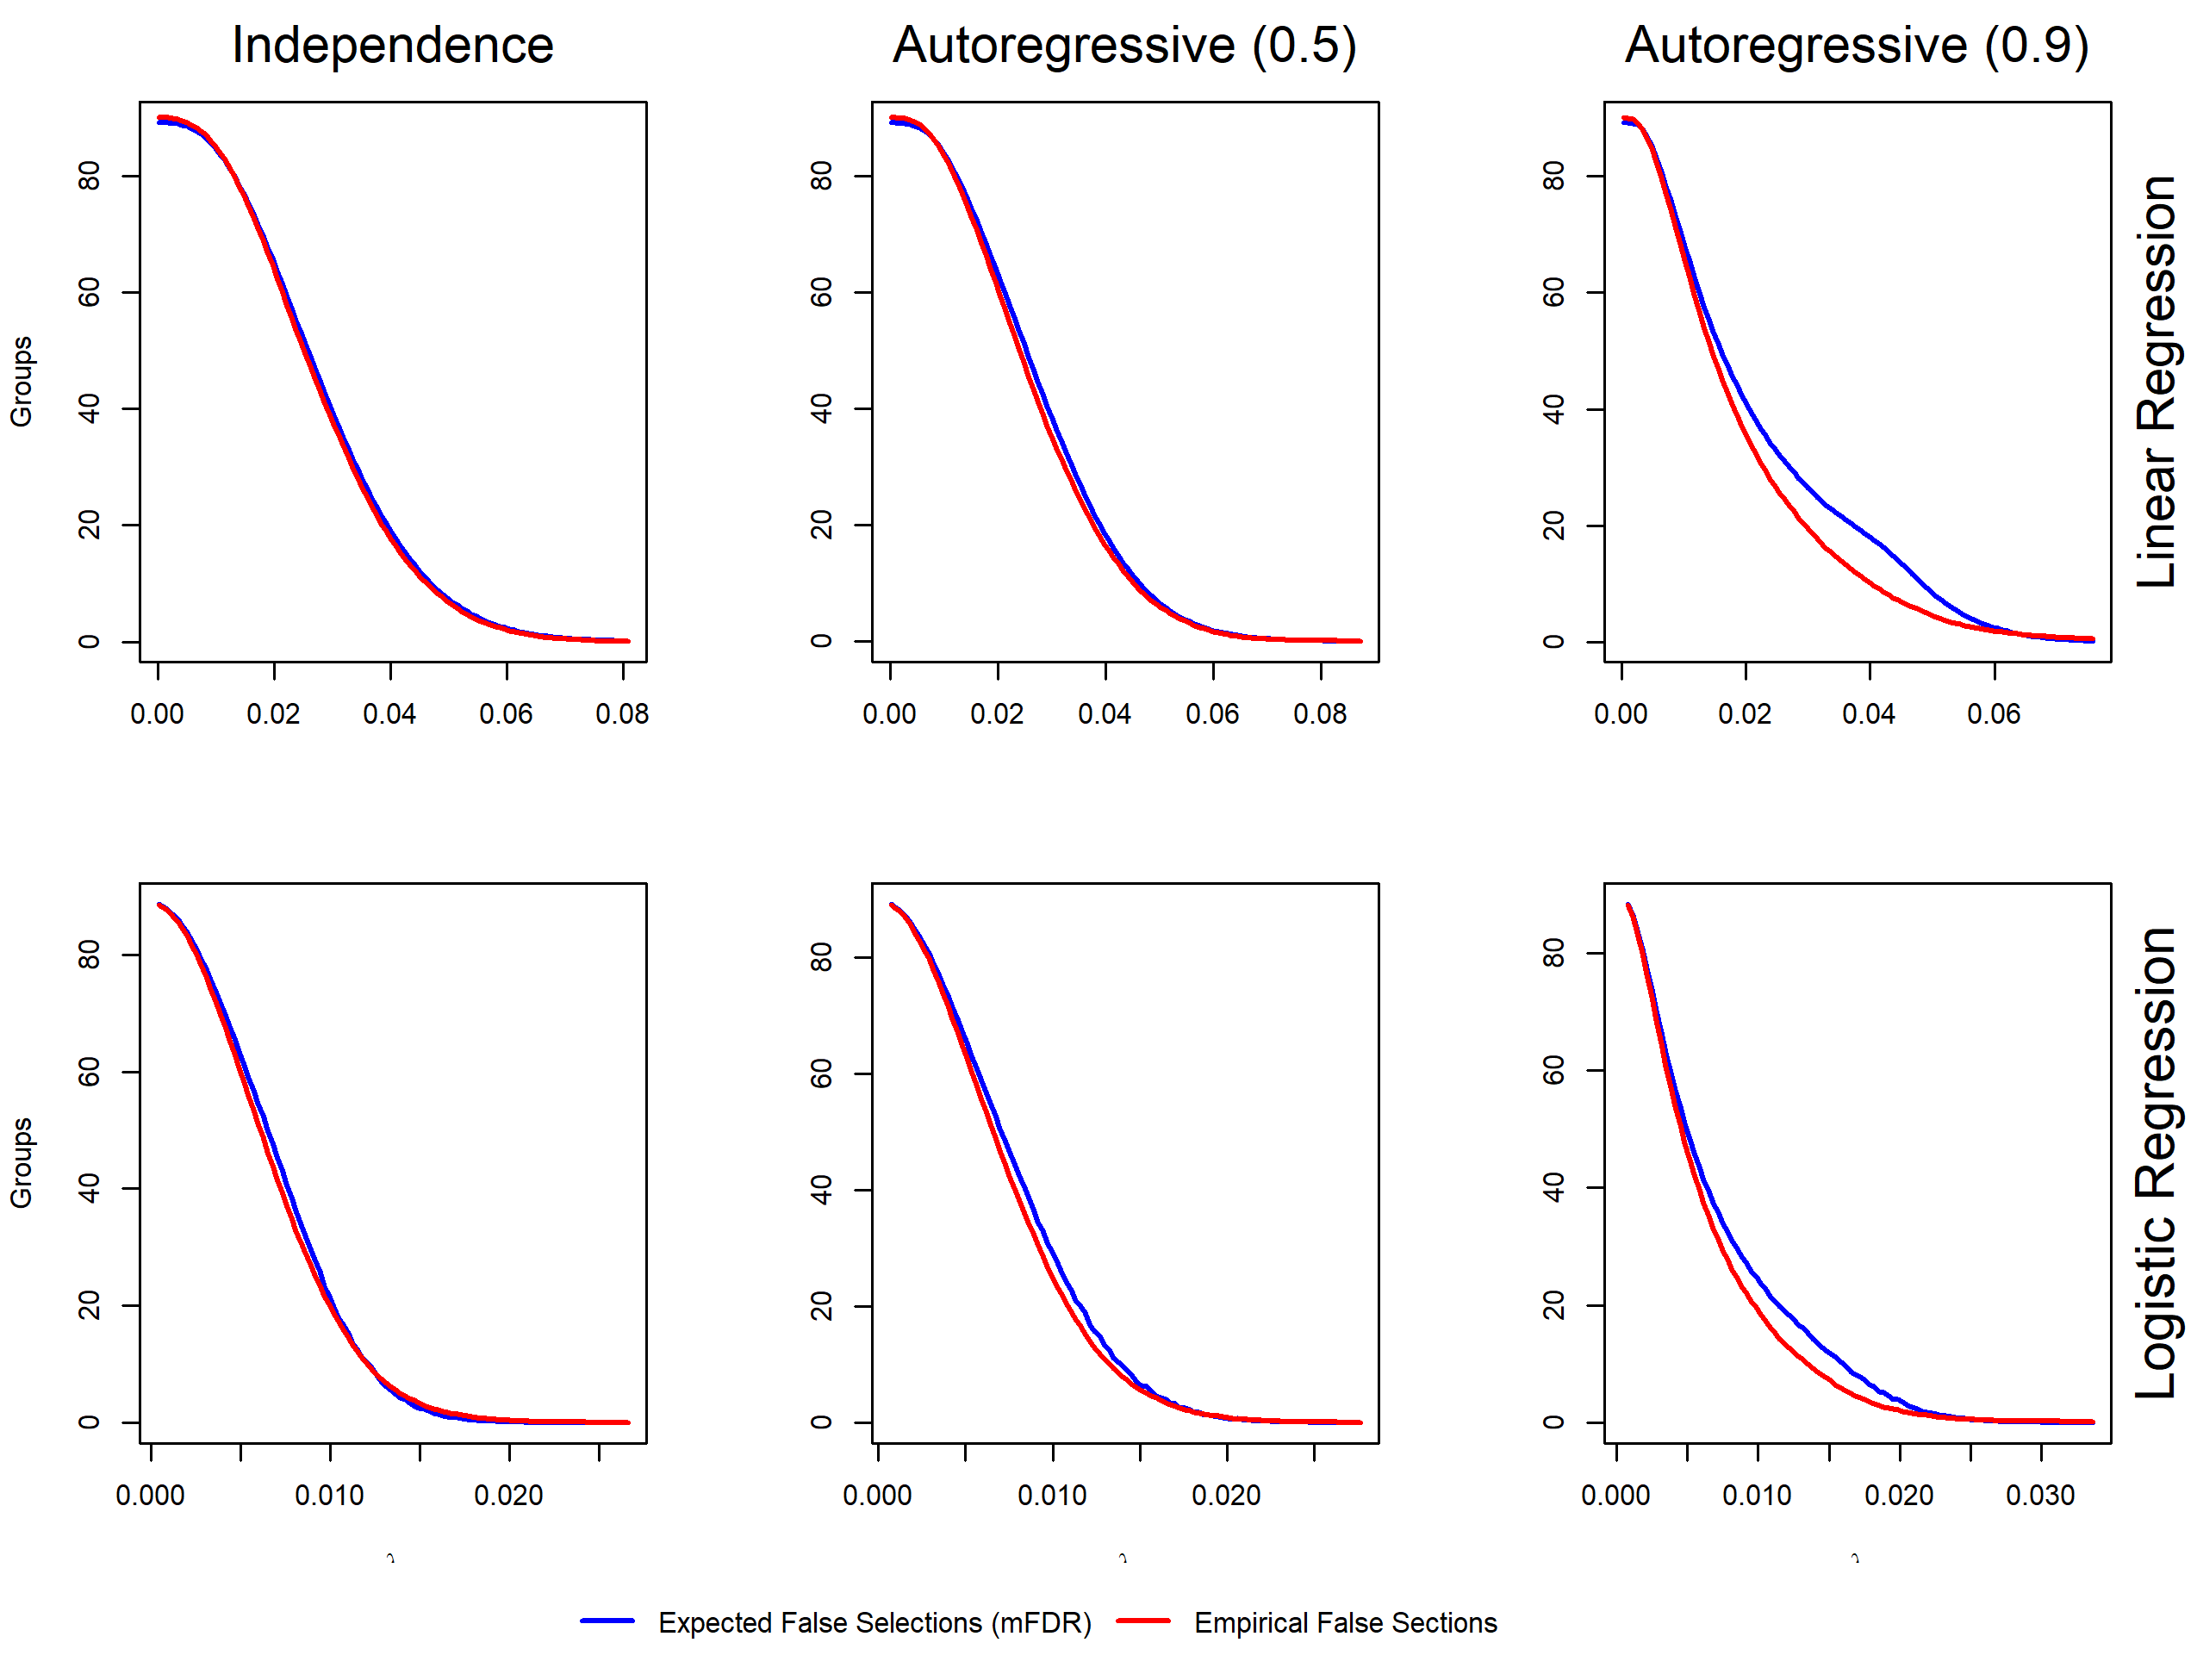
\includegraphics[width=.9\textwidth]{Fig1.png}
  \caption{\label{Fig:lseq} Comparison of the average expected and empirical number of marginal false discoveries along a sequence of $\lambda$ values.}
\end{figure}


In the linear regression setting, under independence, Figure~\ref{Fig:lseq} demonstrates that the expected number of false selections very tightly resembles the empirical number, with only a very slight degree of over-estimation induced by incidental correlations between the columns of $\X$.  As groups become more correlated, the estimates provided by  Equation~\ref{eq:Mfdr} become more conservative.  However, even for $\rho = 0.9$ at the value of $\lambda$ exhbititng the greatest discrepency Equation~\ref{eq:Mfdr} on average suggests only YYY more false discoveries than tend to actually occur, a diference of ZZZ percent.  Results are similar in the logisitic regression setting.  

Focusing on the independence correlation structure and varying $n \in \{200, 400, 600, 800, 1000\}$, we can evaluate the role of sample size in the accuracy mFDR estimates from Equation~\ref{eq:Mfdr}.  Figure~\ref{Fig:conv} displays the mean difference between the estimated and empical false discovery rate, which is defined as $\tfrac{\# \text{Noise selections}}{\# \text{Total selections}}$, when selecting the smallest value of $\lambda$ with $\widehat{\text{Mfdr}} \leq 0.10$ along a fixed sequence across 400 simulation iterations.  As the sample size increases, the discrepency between mFDR and the nominal rate diminishes towards zero.

\begin{figure} [!htb]
 \centering
  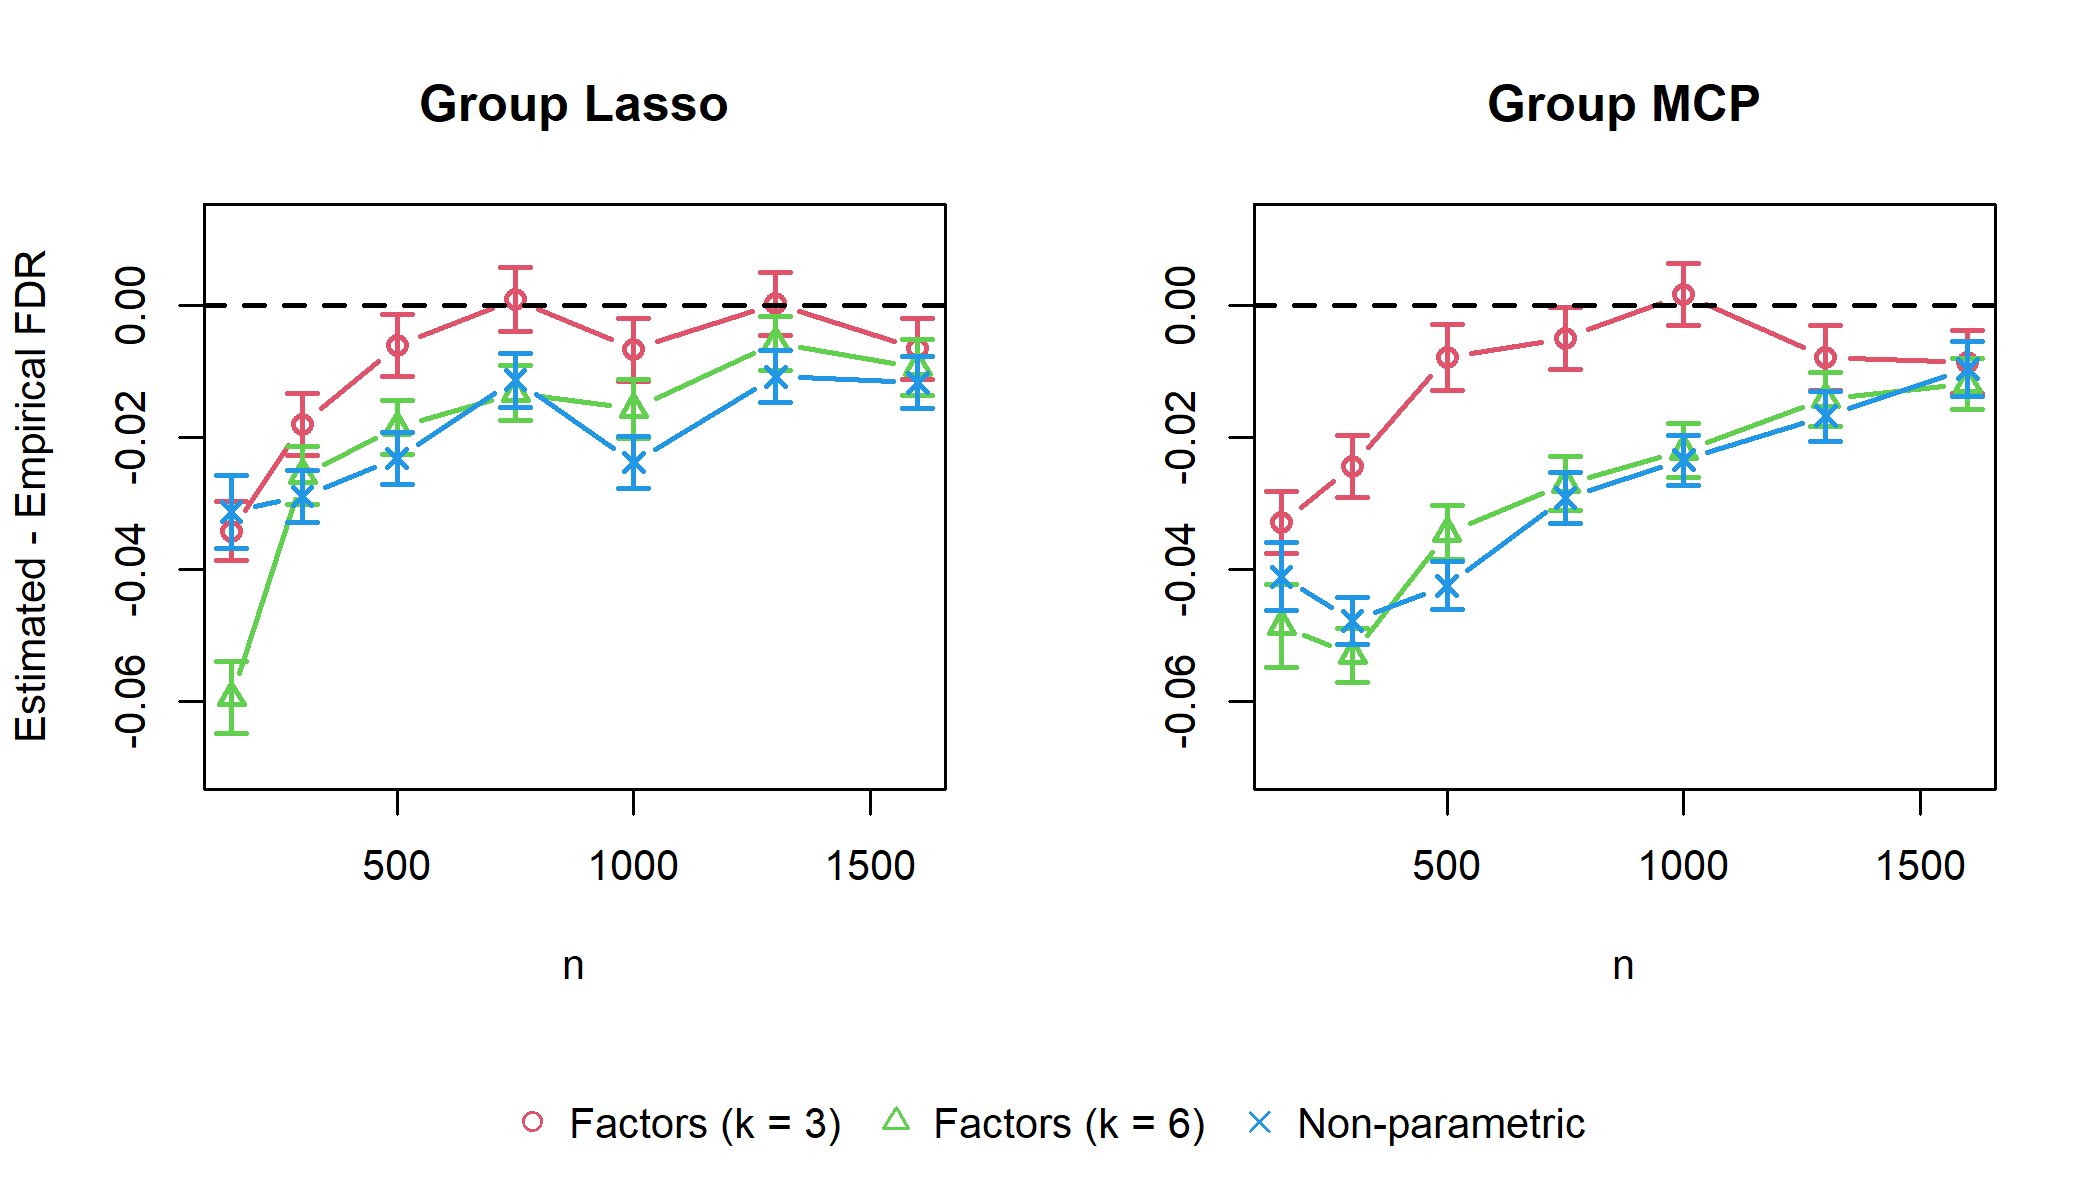
\includegraphics[width=.9\textwidth]{Fig2.png}
  \caption{\label{Fig:conv} Tightness of the $\mFDR$ upper bound as $n$ increases.}
\end{figure}


Figure~\ref{Fig:conv} also demonstrates the compatibility of the mFDR method with the group MCP penalty.  While the group selections and coefficient estimates under this penalization scheme tend to differ from those of the group lasso, the performance of the mFDR estimator remains consistent, if not slightly improved due to more accurate estimation of $\bb$.

\subsection{Comparison with other regression-based methods}

Our third simulation experiment explores the true positive rate of Mfdr approach in comparison with other existing methods for controlling the false discovery rate in the context of group-level selection.  We consider the following competing approaches:

\begin{itemize}[leftmargin=*, labelindent=0.5cm]
\item Forward selection with selective inference
\item Data-splitting
\end{itemize}

\subsection{Comparison with cross-validation}


\subsection{Comparison with univariate methods}

\section{Real data case study}

\subsection{Data}

Lung cancer is among the leading causes of death in the United States and the world, with a high mortality rate that is in part due to a lack of effective diagnostic tools while the disease is still in its early stages. \citet{Spira2007} studied the histologically normal bronchial epitheliums of smokers, collecting RNA expression data for $p = 22,215$ genetic features using Affymetrix HG-U133A microarrays.  Of the $n = 192$ participants, 102 were cases who had already developed lung cancer and 90 were controls who had not developed lung cancer.  The goal of the study was to determine whether gene expression data obtained at bronchoscopy from smokers with suspicion of lung cancer could be used as a lung cancer biomarker.

\subsection{Methods}

In our analysis we consider several different analysis approaches using the genetic data to predict case-control status. Our primary approach applies a basis expansion with 4 degrees of freedom to each genetic feature, thereby creating a new desing matrix, $\tilde{X}$, containing 88,860 columns which correspond to 22,215 groups of size $K_j = 4$.  The $\mFDR$ estimator proposed in \ref{eq:Mfdr_glm} is then used to select a group lasso model that controls the marginal false discovery rate.  

For comparison, we perform traditional large scale univariate testing approach where seperate logistic regression models are fit corresponding to each genetic feature, which is then summarized using a likelihood-ratio test comparing its fit to an intercept-only model.  The Benjamini-Hochberg procedure is then applied to the resulting set of $p$-values to control the false discovery rate at 10\%.   This is done separately using both the original design matrix $\X$, and the expanded design matrix $\tilde{\X}$.  We also analyze the data without performing basis expanasion by fitting a lasso regression model using the binomial likelihood and applying the methods of \citet{Miller2019} to control the false discovery rate.  Finally, we also include selection results for the penalized regressions models favored by 5-fold cross-validation.

\subsection{Results}

\begin{table}[htb!]
\centering
\caption{\label{Tab:case-studies} A summary of various analysis approaches applied to the Spira data. S = number of selections.  mFDR = estimated marginal false discovery rate (\%). MCE = cross-validated misclassification error (\%).}
\vspace{.2cm}
\begin{tabular}{l l l r r r}
  \hline
  Method & Design Matrix & $\lambda$ & S & mFDR & MCE \\
  \hline
  lasso & $\X$ & CV & 55 & 100\% & 24.5\% \\
  lasso & $\X$ & mFDR & 10 & 7.8\%  & 31.8\% \\
  group lasso & $\tilde{X}$ & CV & 45 & 53.4\% & 25.5\% \\
  group lasso & $\tilde{X}$  & mFDR & 21 & 5.6\% & 27.1\% \\
  large-scale testing & $\tilde{X}$  & - & 12,902 & 10.0\% & - \\
  large-scale testing & $\X$ & - & 2,426 & 10.0\% & - \\
  \hline
\end{tabular}
\end{table}

Table~\ref{Tab:case-studies} summarizes the outcome each analysis approach applied to the Spira dataset.  Among penalized regression approaches, the lowest cross-validated misclassification error is obtained by applying the ordinary lasso to the unexpanded design matrix; however, the estimated $\mFDR$ of this model is 100\%.  Because the $\mFDR$ bound is inherently conservative, an estimate of 100\% doesn't necessarily indicate that all of these selections are noise; however, it does suggest that we cannot be confident in the reliability of these selections. For the ordinary lasso, controlling the marginal false discovery rate at 10\% would limit the number of genetic features selected to only 10 while at the same time substantially increasing the cross-validated misclassification error.  In contrast, when applying the group lasso to the expanded design matrix, 21 features can be selected while controlling the marginal false discovery rate below 10\% while achieving a misclassification error that is much closer to the minimum achieved by the ordinary lasso. 

Comparing the number of selections made by the regression-based methods in Table~\ref{Tab:case-studies} to the results of large-scale testing highlights a key advantage of the $\mFDR$.  Although all of these methods are based the same marginal perspective on false discoveries, regression-based methods tend to naturally limit the number of highly correlated features that are deemed significant.  That is, in situations where a large number of features are strongly related with both each other and the outcome, penalized regression tends to select only a single representative from the group, while large-scale testing will select all of them.  In applications such as this one, large-scale testing can result in an overwhelming amount of ``leads" that researchers must then filter, group, or assess manually, while regression-based approaches $\mFDR$ tend to yield a more managable set of features with less redundancy. 

\begin{figure} [!htb]
 \centering
  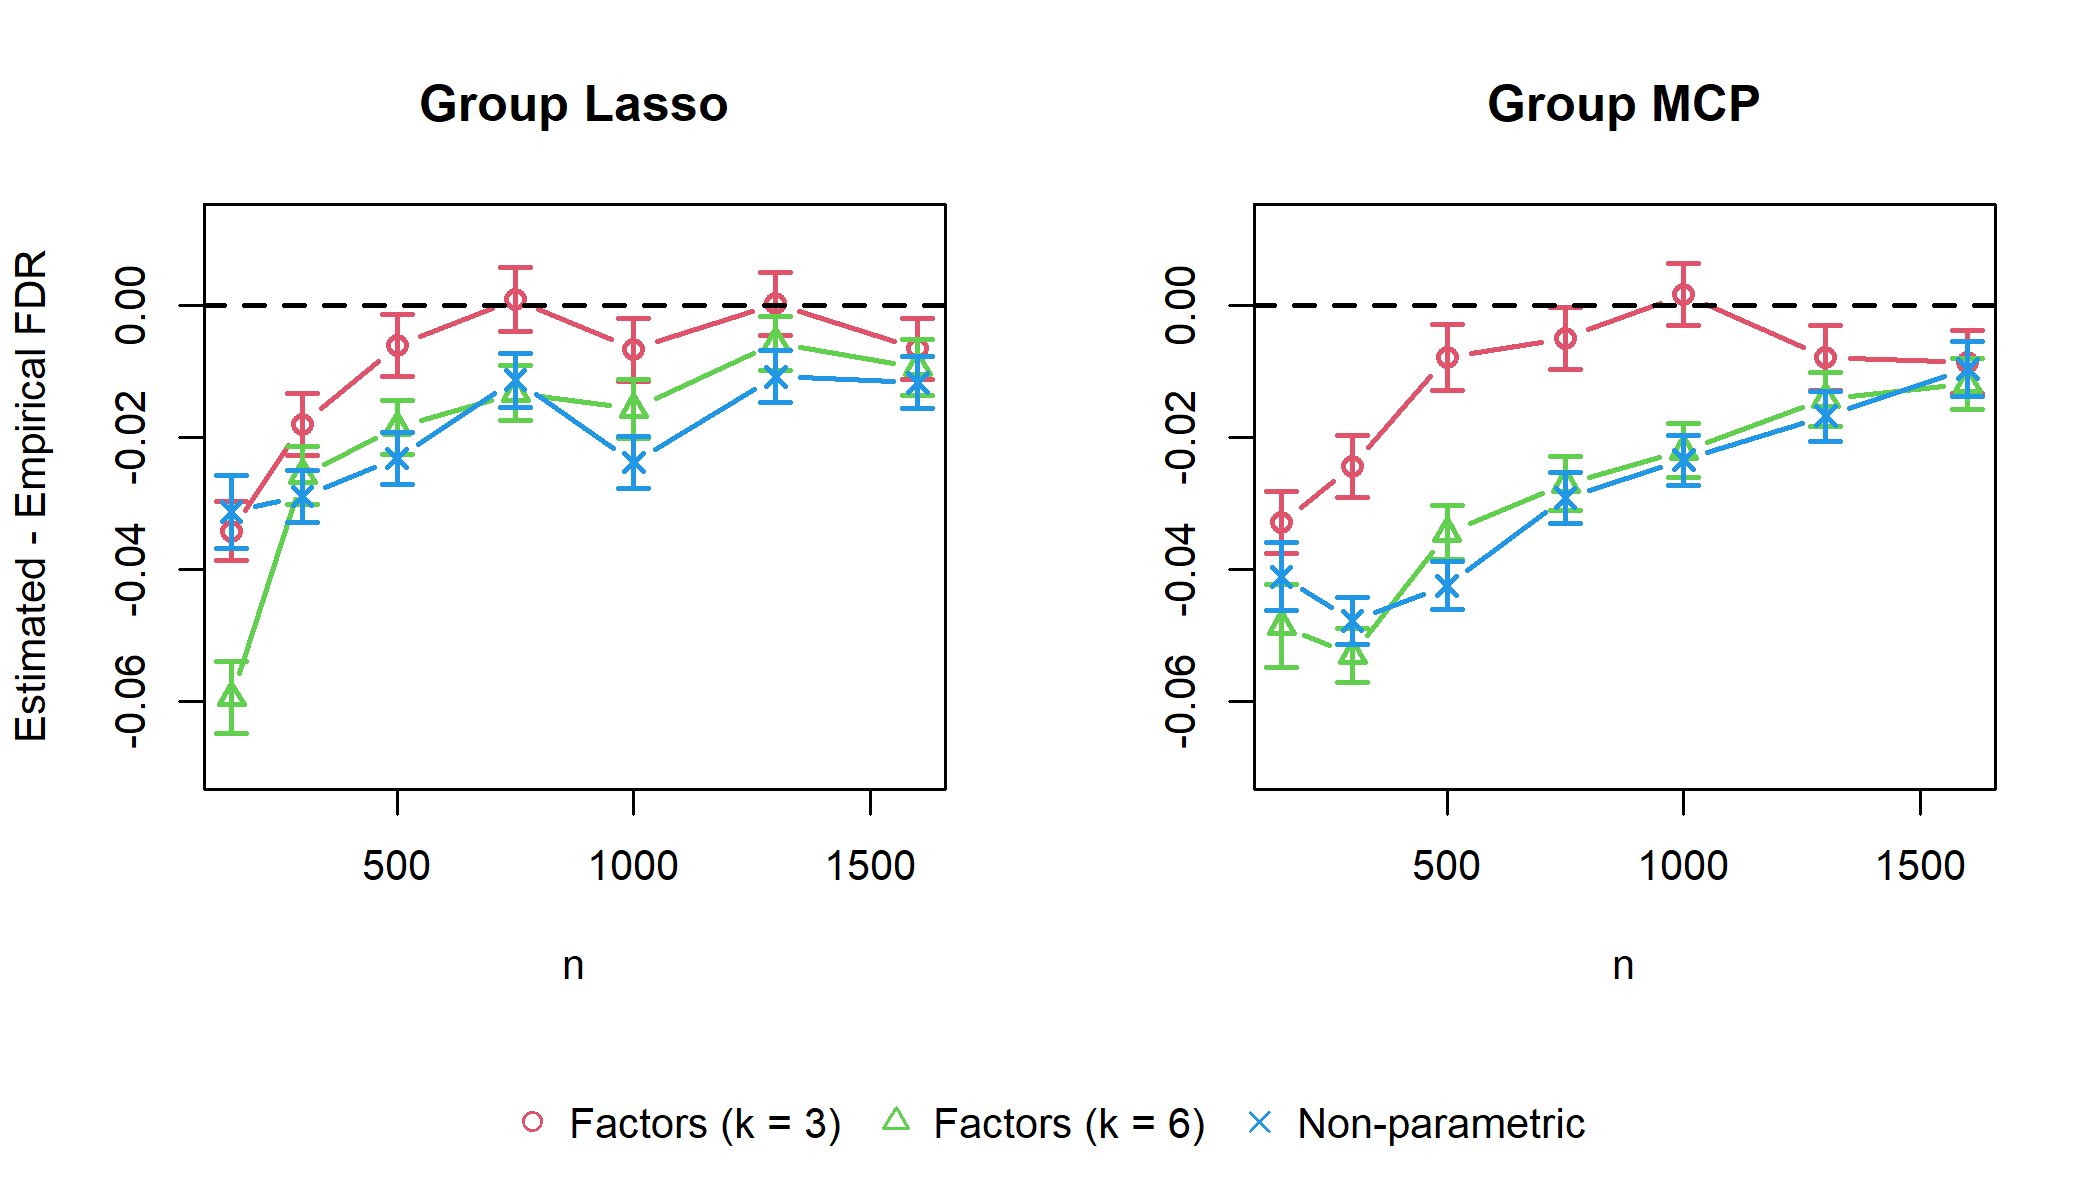
\includegraphics[width=.9\textwidth]{Fig3.png}
  \caption{\label{Fig:casestudy} Group lasso modeling results for the Spira case study.  The left panel displays the cross-validated misclassification error for the models corresponding to various values of a decreasing sequence of $\lambda$, while the right panel shows the total number of selections alongside the expected number of false discoveries for these models.  The model favored by cross-validation marked by a dotted vertical line, while the most inclusive model with an estimated marginal false discovery rate less than 10\% marked by a dashed vertical line. }
\end{figure}

Figure~\ref{Fig:casestudy} provides a more detailed look at the results of the group lasso modeling approach.  The left panel displays the cross-validated misclassification error ($\pm 1$ standard error) for the models corresponding to various values of a decreasing $\lambda$ sequence, demonstrating a wide range of models that achieve statistically similar levels of accuracy.  The right panel shows the expected number of false discoveries, calculated using the estimators in \ref{eq:Mfdr_glm}, and the total number of selections for each of these models.  Together these plots can be used to selection a suitable tradeoff between model accuracy and false discovery rate control.  In this application, the improvements in misclassification error when the penalty parameter is decreased below 0.07 are relatively small and come at the cost of a substantial increase in the expected number of false discoveries present in the corresponding models.

\section{Discussion}

\bigskip

\noindent {{\bf Supporting information}}

\noindent Data and source code to reproduce all results and figures are available at \url{https://github.com/remiller1450/grp_mfdr_paper}.